\subsection{}
The monopolist has perfect information in a price discriminating monopoly.\\
In order for price discrimination to exist, 4 scenarios must exist:
\begin{enumerate}
    \item The demand curve must be downward sloping.
    \item Monopolists need to be able to segment their markets. (i.e. student discounts)
    \item Consumer response (elasticity) must be different.
    \item Monopolists need to prevent resale.
\end{enumerate}
Marginal Revenue will be different in a price discriminating monopoly.\\
The demand curve is equal to marginal revenue.\\
The price discriminating monopoly produces more than a single price monopoly.\\
The price discriminating monopoly produces the same amount as a perfectly competitive market.\\
The price discriminating monopoly price charged is a range between the demand curve and the marginal cost curve.\\
Price discriminating monopoly will always be more profitable than a single price monopoly.\\
Total revenue in a price discriminating monopoly is calculated by adding the total revenue of each segment. It is not simply P $\times$ Q\\
MR = D.
\begin{figure}[H]
    \centering
    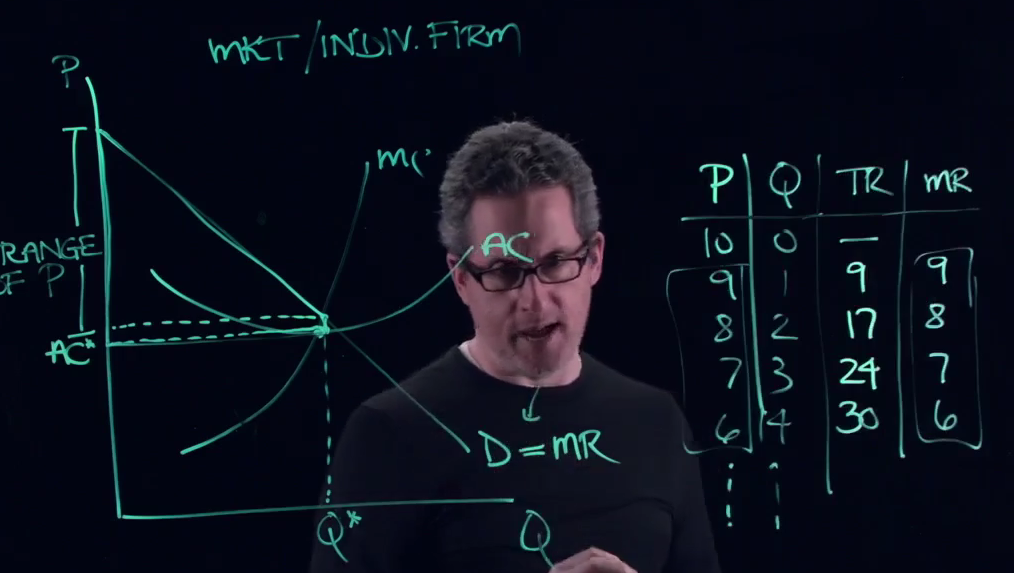
\includegraphics[width=0.5\textwidth]{Chapter10/PriceDiscrimination.png}
    \caption{Price Discriminating Monopoly}
    \label{fig:pricediscriminating}
\end{figure}
The more inelastic the demand curve, the higher the price charged and higher the profit.\\